%************************************************
\section{几个有意思的工具}
\begin{frame}
  \frametitle{TeXFriend}
  \begin{enumerate}
    \item<2-> 南开大学孙文昌开发,WinEdt自带。
    \item<3-> TeXFrined提供几千个LaTeX字符的自动输入。
  \end{enumerate}
  \begin{center}
    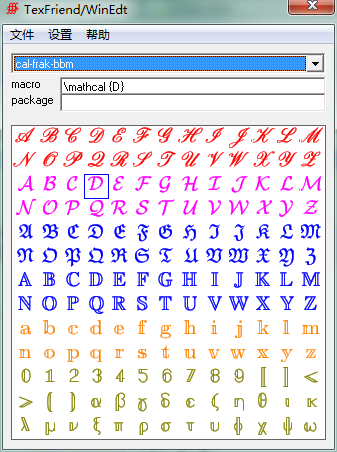
\includegraphics[width=0.4\textwidth]{texfriend.png}
  \end{center}
\end{frame}

\begin{frame}
  \frametitle{LYX}
  \begin{center}
    
\includegraphics[width=0.3\textwidth]{lyx.png}
  \end{center}
  \begin{enumerate}
    \item<2-> LyX是一个“所见即所指”(what you see is what you mean)的文件编辑软件。
    \item<3-> LyX利用\LaTeX{}来排版。
    \item<4-> 通过CJK-LyX提供中文支持。
    \item<5-> 可以生成\LaTeX{}文件和 PostScript 文件。
  \end{enumerate}
\begin{center}
    \footnotesize{\url{http://wiki.lyx.org/uploads/LyX/Screencasts/LyXIntroPalette.htm}}
\end{center}
\end{frame}

\begin{frame}
  \frametitle{Word2TeX}
  \begin{enumerate}
    \item<2-> 在Word中编辑文章
    \item<3-> 安装Word2TeX软件
    \item<4-> 将Word文档转化为TeX文件
    \item<5-> 对生成的TeX文件修改
    \item<6-> 再用LaTex编译为PDF文档
  \end{enumerate}
  \begin{center}
    
\includegraphics[width=0.3\textwidth]{word2tex.png} \qquad
    
\includegraphics[width=0.3\textwidth]{tex2word.png}
  \end{center}
\end{frame}